\section{E-Mail Template of the Awareness Part}
\label{a:mail}
\lstset{language=html}
\begin{lstlisting}
<html>
  <head>
    <title>Anti Phishing Education</title>
  </head>
  <body>
    <p>Dies ist eine automatisch generierte E-Mail im Rahmen einer Anti-Phishing Education App. Falls diese nicht angefordert wurde, bitte ignorieren.</p>
    <p>Ansonsten geht es hier weiter:</p>
    <p>Wie du im Absender siehst, hast du dir gerade selbst eine E-Mail mit gefälschtem Absender geschickt. Hier ist außerdem dein Freitext:</p>
    <p>{$usermessage}</p>
    <p>Für einen Angreifer ist es ebenso einfach automatisierte E-Mails mit gefälschtem Absender und Inhalt zu verschicken. Meist enthalten diese einen Link zu einer Webseite, genau wie diese E-Mail.</p>
    <p>Um mit der App fortzufahren, klicke auf den folgenden Link.</p>
    <p><a href="http://pages.no-phish.de/maillink.php">http://www.google.com</a></p>
    <p>Viele Grüße,</p>
    <p>Dein NoPhish Team</p>
  </body>
</html>
\end{lstlisting}

%===========================================
\section{URL Generation Process}
\label{s:url_generation}
%===========================================
When playing the app (level 2-9) the user has to categorize a given URL as a phish or valid URL.
We decided against a fixed set of examples for the URLs because depending on the set size it might happen that a user keeps being confronted with the same URLs.
We believe it is essential for the user to be faced with as many different URL examples as possible.
Therefore, we decided to generate the URLs rather than composing a fixed list.
Next, we lay out the URL generation process and cover further interesting aspects of the URL generation in the subsequent sections.
\subsection{Derive Phishing URLs from Legitimate Example URLs}
To present attacked URLs to the user we found it most realistic to take valid URLs and apply the covered attacks to them.
For this purpose, we needed a set of legitimate URLs.
To build this set we used Alexa~\cite{alexa} to select various domains from the top 100 website vendors of Germany.
Then, we visited each of these websites, navigated through them and picked about 3-6 URLs for each domain we had previously selected.
We strived to balance the number of short and long URLs.
Given a list of valid URLs an attack can be applied whenever required.
In the following we discuss how this is accomplished in our implementation.
\begin{description}[leftmargin=0cm]
\item[Generate a List of Attacks for Each Level:] When starting a new level we generate a list of attacks with which the user needs to be confronted.
\item[Select a Valid URL:] Whenever a new URL is to be shown to the user we first randomly select a valid URL from the aforementioned set.
\item[Modify Valid URLs with a Generator:] Then we apply a generator to the URL that does not invalidate the URL but modifies it (cf. \autoref{s:apply_generator}).
\item[Apply an Attack:] After that we select a random attack from the previously built list and apply it to the selected valid URL.
\item[Repeat in Case Attack was not Possible:] In some cases applying a specific attack to a given URL is not possible. For example, in homograph attacks the replacement of an ``i'' with another letter in a URL which does not contain an ``i'' will fail. In these situations we have to retry.
\end{description}

\subsection{Number of Phishes and Repetitions per Level}
%\textbf{Was zur historie?}
The types of spoofed URLs the user is faced with depends on the level.
Each level introduces one ore more attacks.
The introduced attacks of each level are layed out in \autoref{s:knowledgetransferperlevel}.
In general, the URLs of each level $n$ are distributed as follows:
\begin{table}[hHtbp]
\centering
\begin{tabular}{|llll|}
\hline
Total number of URLs&$u$&$6+2*n$&Starting with 6 URLs each level has 2 more URLS.\\
Number of phishes&$p$&$u/2$&Half of the URLs are phishes.\\
Number of repetitions&$r$&$\left\lfloor p/2 \right\rfloor$&Half of the phishes are repetitions.\\
\hline
\end{tabular}
\caption{Distribution of URLs per level}
\label{t:levelurls}
\end{table}
Repetitions are also included into the list of attacks to be applied which is created upon start of each level.
The list of repetitions is filled up as follows: every level has exact one attack repetetion for each previous level. The rest of the repetitions is filled up randomly. This way, we assure that at least one example of each previous level is represented by the attack repetitions. All remaining phishes are new attacks.
There are two main exception to these rules:
\begin{description}[leftmargin=0cm]
\item[Level 1:] In level 1 the user is only confronted with valid URLs and has to select the domain.
To prevent the user from getting bored we only present 5 URLs in this level.
None of them is a phish.
\item[Level 1+2:] The first level that contains repetitions is level 3 because level 2 introduces the very first spoofing attack. Consequently, level 1 and level 2 do not have repetitions.
\end{description}

%The generated list of attacks also contains a special attack that does no real attack. This is to %simplify the URL generation. When we generated the list of attacks we save it for later reference.

\subsection{Modify Legitimate URLs with a Generator}
\label{s:apply_generator}
We were unsure whether we had collected sufficient valid URLs.
 For this reasons, we prepared a way to automatically modify the URLs in such a way that they remained valid URLs. 
Some ideas were to add subdomains or path strings to the URL. Queries or fragments would also  be possible. 
Later we found out that it was currently not required to implement such generators since our set contained enough URL examples. 
Yet, if we should realize in future that these URLs are not enough we have this scheme in place.
\subsection{Re-Apply an Attack in Case of Wrong User Answer}
After generating a valid URL we choose a random attack from the previously built set of attacks and apply it to the URL. We also store which attack we currently apply. This is important in case  the user fails to give a correct answer to the current URL. In this situation we will simply readd this attack to the set of attacks.
This way, we assure that the attack, which the user failed to identify, is repeated later in this level.
%\subsection{Repeat in Case Attack was not Possible}
%There are combinations of base-URL and attack where the attack doe's not alter the URL.
%Therefore it would be impossible for the user to detect the Attack and he will be confused and %might stop using the app.
%In this situation we repeat the whole URL generation process until we find a matching URL.

\section{Questionnaire of Study for Input}
\label{s:presurvey_form}
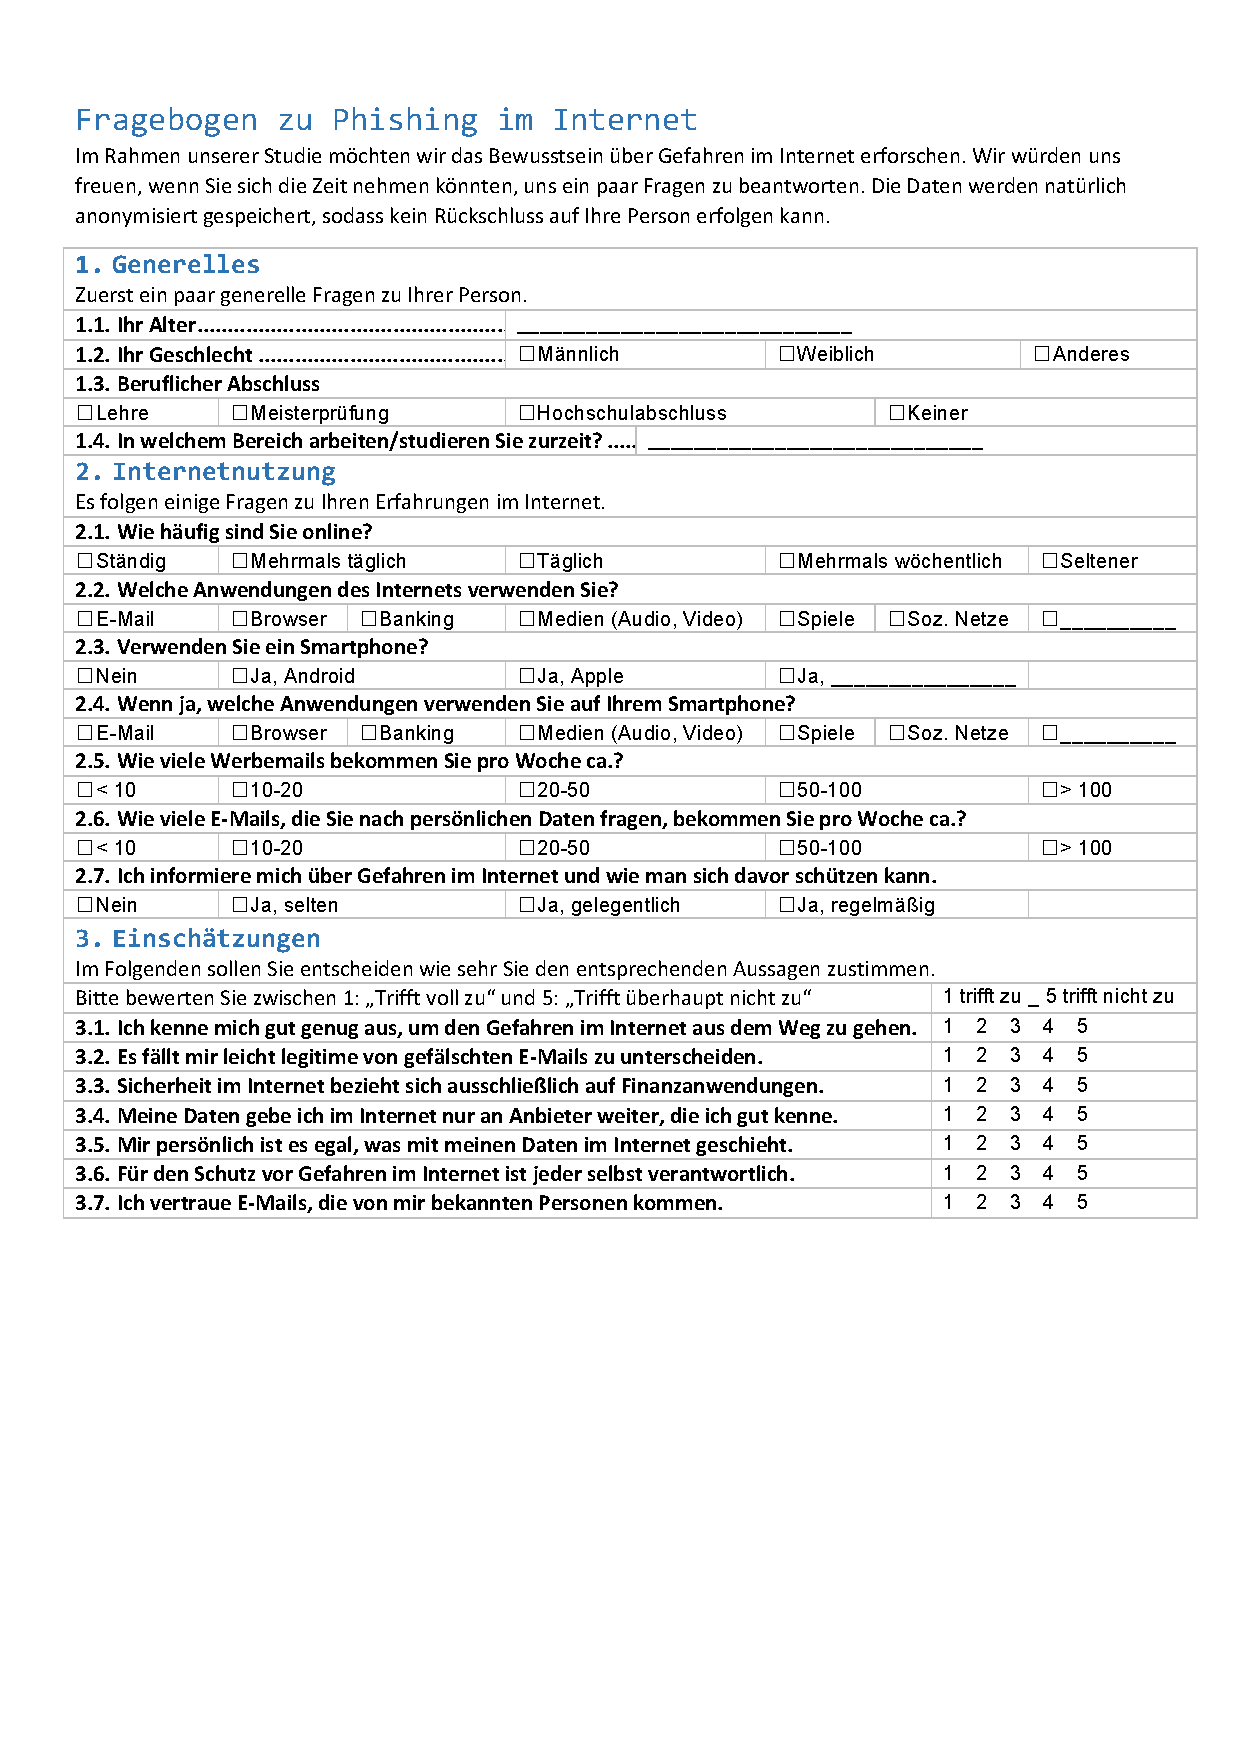
\includepdf[pages=-,frame,scale=0.8]{graphix/presurvey.pdf}


\section{Final Study}

\subsection{Participant Recruitment}
\label{s:participant_recruitment_texts}

Sehr geehrte/r ....,
\newline
\newline
wir, Clemens Bergmann und Gamze Canova, sind Studenten des Fachbereichs Informatik an der TU Darmstadt und arbeiten zur Zeit unserer Masterthesis zum Thema Internetsicherheit.
\newline
\newline
Nun sind wir an dem Punkt angekommen, an dem wir eine Benutzerstudie (6.1.-11.1.2014) durchf\"{u}hren m\"{u}ssen, f\"{u}r die wir Teilnehmer suchen. Wir w\"{u}rden uns sehr freuen, wenn Sie uns hierbei unterst\"{u}tzen k\"{o}nnten. W\"{a}re es m\"{o}glich, den angeh\"{a}ngten Flyer mit dem unten stehenden Anschreiben, an Ihre StudentInnen und/oder Wissenschaftliche MitarbeiterInnen  weiterzuleiten? Wir wissen, dass es schwierig sein k\"{o}nnte potentielle Teilnehmer kurz vor Weihnachten zu erreichen, jedoch k\"{o}nnen wir jede Unterst\"{u}tzung gebrauchen und w\"{u}rden uns \"{u}ber diese sehr freuen.
\newline
\newline
Wir bedanken uns im Voraus herzlich f\"{u}r Ihre Bem\"{u}hungen und w\"{u}nschen Ihnen erholsame und besinnliche Festtage.
\newline
\newline
Mit freundlichen Gr\"{u}{\ss}en, \newline
Clemens Bergmann und Gamze Canova
\newline
\newline
Text f\"{u}r Weiterleitung:
Im Rahmen unserer Masterarbeit haben wir eine Spiele-App entwickelt, die fachfremde Benutzer \"{u}ber Internetsicherheit informiert.  Diese App soll im Rahmen einer Benutzerstudie getestet werden. Hierzu brauchen wir deine Hilfe. Die Studie wird in Gruppen zu ca. 5 Personen in der zweiten Januarwoche (6.-10.) in Darmstadt stattfinden und insgesamt ca. 90 Minuten in Anspruch nehmen.  Der/Die Beste der Gruppe gewinnt einen Amazon-Gutschein im Wert von 20\euro.  Einzige Voraussetzung f\"{u}r die Teilnahme ist, dass du Erfahrung mit der Benutzung eines Smartphones hast. Bei Interesse oder Fragen erreicht ihr uns unter netstudy@cased.de. 


\includepdf[pages={1},frame,scale=0.8]{graphix/flyer.pdf}


\subsection{Explanatory Texts of Each Study Step}
In order to ensure that the studies of small groups remain comparable we read all explanatory texts to the participants. 
This section provides a collection of these texts

\subsubsection{Welcome and Introduction to Consent Form and General-Survey Before}
Herzlich willkommen zu unserer Benutzerstudie.
Danke, dass ihr euch die Zeit genommen habt uns zu unterst{\"u}tzen.
Bitte bedient euch an den S{\"u}{\ss}igkeiten und dem Wasser auf den Tischen.
W{\"a}hrend der Studie werden wir die Erl{\"a}uterungen vorlesen. Damit wollen wir sicherstellen, dass alle Durchl{\"a}ufe vergleichbar bleiben. 
\newline
\newline
Wir w{\"u}rden euch gerne fragen, ob es in Ordnung f{\"u}r euch w{\"a}re, wenn wir das Gewinnspiel ein bisschen ab{\"a}ndern: wir haben n{\"a}mlich festgestellt, dass es in der Studie in Ausnahmef{\"a}llen passieren kann, dass ihr nicht die gleichen Chancen habt zu gewinnen. Daher w{\"u}rden wir am Ende den Amazon-Gutschein gerne verlosen. Ist das f{\"u}r alle in Ordnung?
Alles klar, super. Dann kanns weiter gehen.
\newline
\newline
In der Studie soll eine App getestet werden, die in Form eines Spiels Benutzern beibringen soll, wie sie sich besser vor Betrug im Internet sch{\"u}tzen k{\"o}nnen. Um das Ganze ein bisschen spannend zu gestalten, wird am Ende die Person ermittelt, die hierbei am besten abgeschnitten hat.
Ziel der Studie ist, die Wirksamkeit der App zu Testen. Hierzu haben wir folgenden Ablauf geplant:
Keine Angst, ihr m{\"u}sst euch nicht die einzelnen Schritte merken, wir erkl{\"a}ren jedes mal was als n{\"a}chstes kommt.
\newline
\newline
Als erstes bekommt ihr zwei Frageb{\"o}gen ausgeteilt.
Der Erste ist eine Einverst{\"a}ndniserkl{\"a}rung, die ihr unterschreiben m{\"u}sst, wenn ihr mitmachen wollt. Auf dem zweiten wird eure Selbsteinsch{\"a}tzung bzgl. eures Wissens zur Internetsicherheit abgefragt.
Im zweiten Teil werden wir an Hand von Beispielen euer Vorwissen zum Thema Internetsicherheit genauer erfassen. Dies dient uns als Basiswert. 
Im dritten Teil werden wir euch Smartphones mit der App austeilen und ihr habt Zeit die App auszuprobieren. 
Dabei sammelt ihr bei dem Spiel Punkte, welche dar{\"u}ber entscheiden, wer von euch vieren das Spiel gewinnt. Dies wird die l{\"a}ngste Zeit in Anspruch nehmen.
Im vierten Teil werden wir euch erneut Beispiele zeigen, um zu erfassen,
in wie weit, die App euch unterst{\"u}tzt. 
Im f{\"u}nften Teil folgt eine "Freispielphase" in der ihr weitere Erfahrungen mit der App sammeln k{\"o}nnt.
Im sechsten Teil folgt ein weitere Fragebogen zur allgemeinen Benutzbarkeit der App.
Anschlie{\ss}end wird der Gewinner ermittelt und (der Amazon-Gutschein verlost) und damit ist die Studie auch beendet. Zuletzt w{\"u}rden wir uns freuen, wenn ihr noch einige Minuten f{\"u}r eine kurze offene Diskussionsrunde bleiben w{\"u}rdet, um eure Anmerkungen loszuwerden.
Soviel zum Ablauf.
\newline
\newline
Bei Fragen oder Problemen mit der App meldet euch einfach und wir kommen zu euch um die anderen nicht unn{\"o}tig zu st{\"o}ren. Wir werden euch bei technischen Problemen oder Bedienungsproblemen helfen. Inhaltliche Fragen k{\"o}nnen wir nicht beantworten weil dadurch der Einfluss der App auf euch nicht mehr gepr{\"u}ft werden k{\"o}nnte.
Ihr habt jederzeit das Recht zu gehen und die Studie abzubrechen. Beachtet aber: Wenn ihr die Studie nicht vollst{\"a}ndig mitmacht, k{\"o}nnt ihr nat{\"u}rlich nicht am Gewinnspiel teilnehmen.
\newline
\newline
Wichtig ist: Bitte bearbeitet alle Fragen und die App alleine. Ihr k{\"o}nnt nichts falsch machen. Beantwortet einfach alle Fragen nach besten wissen. Damit helft ihr uns am meisten. Wenn ihr mit dem Ausf{\"u}llen jeweils fertig seid gebt uns die Frageb{\"o}gen einfach zur{\"u}ck.
Habt ihr dazu noch Fragen?
\newline
\newline
Bevor es jetzt losgeht, wollten wir noch darauf hinweisen, dass die Studie ab jetzt ca. 1 Stunde dauern wird. Wegen des Studienaufbaus ist es leider nicht m{\"o}glich sie zwischendurch kurz zu unterbrechen, daher nutzt jetzt bitte die Gelegenheit, falls ihr kurz raus m{\"u}sst.
\newline
\newline
Ok, bevor es losgeht w{\"u}rden wir euch gerne darum bitten, eure Handys auf lautlos zu schalten und auch die Vibration auszustellen. Danke.
Hier sind erst einmal die Einverst{\"a}ndniserkl{\"a}rungen. Wenn ihr damit fertig seid, geben wir euch den zweiten Fragebogen.

\subsubsection{Introduction to Website-Survey Before}
Nachdem wir nun wissen was ihr vor dieser Studie {\"u}ber Internetsicherheit wusstet, k{\"o}nnen wir nun etwas konkreter werden.
Bei der App handelt es sich um ein Spiel welches euch speziell Tips zum Thema Phishing gibt.
Phishing ist ein Betrugsversuch. Hierbei spielt der Betr{\"u}ger dem Benutzer vor jemand anderes zu sein. Das Ziel des Betr{\"u}gers ist, dem Benutzer pers{\"o}nliche Informationen zu entlocken. Meistens macht er das {\"u}ber gef{\"a}lschte Webseiten.
\newline
\newline
Im n{\"a}chsten Fragebogen zeigen wir euch daher ein paar Webseiten. Ihr m{\"u}sst entscheiden, ob diese gef{\"a}lscht oder legitim sind.
F{\"u}r unsere Auswertung ist es wichtig, dass ihr die Seiten in der vorgegebenen Reihenfolge beantwortet und nicht zur{\"u}ck bl{\"a}ttert, auch wenn euch im Nachhinein etwas auff{\"a}llt. Schaut lieber zweimal hin.

\subsubsection{Introduction to Playing App}
So, jetzt ist die App an der Reihe.
Wir teilen euch jetzt die Smartphones aus.
Zus{\"a}tzlich teilen wir euch einen Zettel aus. Darauf k{\"o}nnt ihr Anmerkungen zur App direkt notieren.
Diesen k{\"o}nnt ihr bis zum Ende behalten und weiterhin Notizen darauf machen. Ihr k{\"o}nnt ihn dann am Ende mit dem letzen Fragebogen abgeben.
\newline
\newline
Jedes Telefon ist mit der Nummer eures Sitzplatzes beschriftet. Bitte verwendet nur euer Telefon.
Auf dem Starbildschirm der Handys befindet sich die App. Sie hei{\ss}t ``NoPhish''.
Wenn wir euch sagen, dass es losgeht, startet die App durch Antippen und w{\"a}hlt im Startmen{\"u} auf den gr{\"u}nen Button, um das Spiel zu starten.
Ihr habt zum Spielen 30 Minuten zeit.
\newline
\newline
Im Laufe der App, werdet ihr nach eurer E-Mail Adresse gefragt. Dazu sind auf den Smartphones speziell f{\"u}r die Studie E-Mail Adressen angelegt worden. Diese werden euch bei der Eingabe in das Feld vorgeschlagen. Bitte w{\"a}hlt diese aus. Bei der Absender-Adresse d{\"u}rft ihr eingeben, was ihr wollt.
\newline
\newline
Es ist nicht m{\"o}glich die App in der Zeit vollst{\"a}ndig durchzuspielen. Spielt einfach so weit ihr kommt.
Wenn wir euch am Ende bescheid geben h{\"o}rt bitte einfach auf die App zu spielen und lasst sie so wie sie ist. Nur so k{\"o}nnen wir eure Punktzahl korrekt ablesen.
Jetzt geht's los. Viel erfolg.


\subsubsection{Introduction to Website-Survey After and Further App Exploration}
Die Zeit ist um. Bitte legt jetzt die Smartphones weg. Wir sammeln sie jetzt ein.
\newline
\newline
Jetz kommt nochmal ein Fragebogen mit Webseiten. Wie vorher sollt ihr darauf entscheiden ob eine Webseite gef{\"a}lscht oder legitim ist. Wenn ihr damit fertig seid gebt den Fragebogen uns wieder zur{\"u}ck.
\newline
\newline
Jetzt teilen wir wieder die Smartphones aus. Wir bitten euch diesmal die anderen Funktionen der App auszutesten. Daf{\"u}r habt ihr dann nochmal 5 Minuten.


\subsubsection{Introduction to General-Survey After}
Zum Schluss nochmal ein Fragebogen zur Benutzbarkeit. Wenn ihr damit fertig seid, gebt ihn bitte zusammen mit eurem Notizzettel wieder ab.

\subsubsection{Issuance of Certificates, Debrief and Goodbye}
Ihr habt es geschafft.
Vielen Dank, dass ihr euch die Zeit genommen habt, die App zu testen.
Haben sich bei euch noch Fragen ergeben?
\newline
\newline
Alles klar, dann kommen wir zur Bekanntgabe des Gewinners vom Spiel.
Gewonnen hat <gewinnername/>, mit <gewinnerpunkte/> Punkten.
Herzlichen Gl{\"u}ckwunsch, du hast am besten abgeschnitten. 
\newline
\newline
Nun kommen wir zur Verlosung des Amazon-Gutscheins. 
<name/> hat den Amazon-Gutschein gewonnen, herzlichen Gl{\"u}ckwunsch. \newline
<Erhaltbest{\"a}tigung unterschreiben lassen/>
\newline
\newline
Allen anderen vielen Dank nochmal f{\"u}r eure Teilnahme.\newline
<Austeilen der Anti-Phishing Awards>
\newline
\newline
Zum Schluss w{\"u}rden wir uns freuen, wenn ihr noch in einer kurzen Diskussionsrunde mitmachen w{\"u}rdet. Diese ist freiwillig. Wer m{\"o}chte jetzt gerne gehen? Sehr sch{\"o}n, danke.
\newline
\newline
Die offene Diskussion w{\"u}rden wir gerne mit einem Diktierger{\"a}t aufzeichnen. Ist das f{\"u}r alle in Ordnung?
\newline
\newline
Nochmal vielen Dank an alle Teilnehmer.
Wir hoffen es hat euch etwas Spa{\ss} gemacht und w{\"u}nschen euch noch einen sch{\"o}nen Tag.
Nehmt euch gerne noch Kekse und Gummib{\"a}rchen f{\"u}r auf den Weg mit.
\newline
\newline
Tsch{\"u}ss

\subsection{Study Forms}
The following pages contain the forms as we used them in the user study. We did not include all example URL but only one exemplary page with an attacked URL.
\label{s:before_survey}
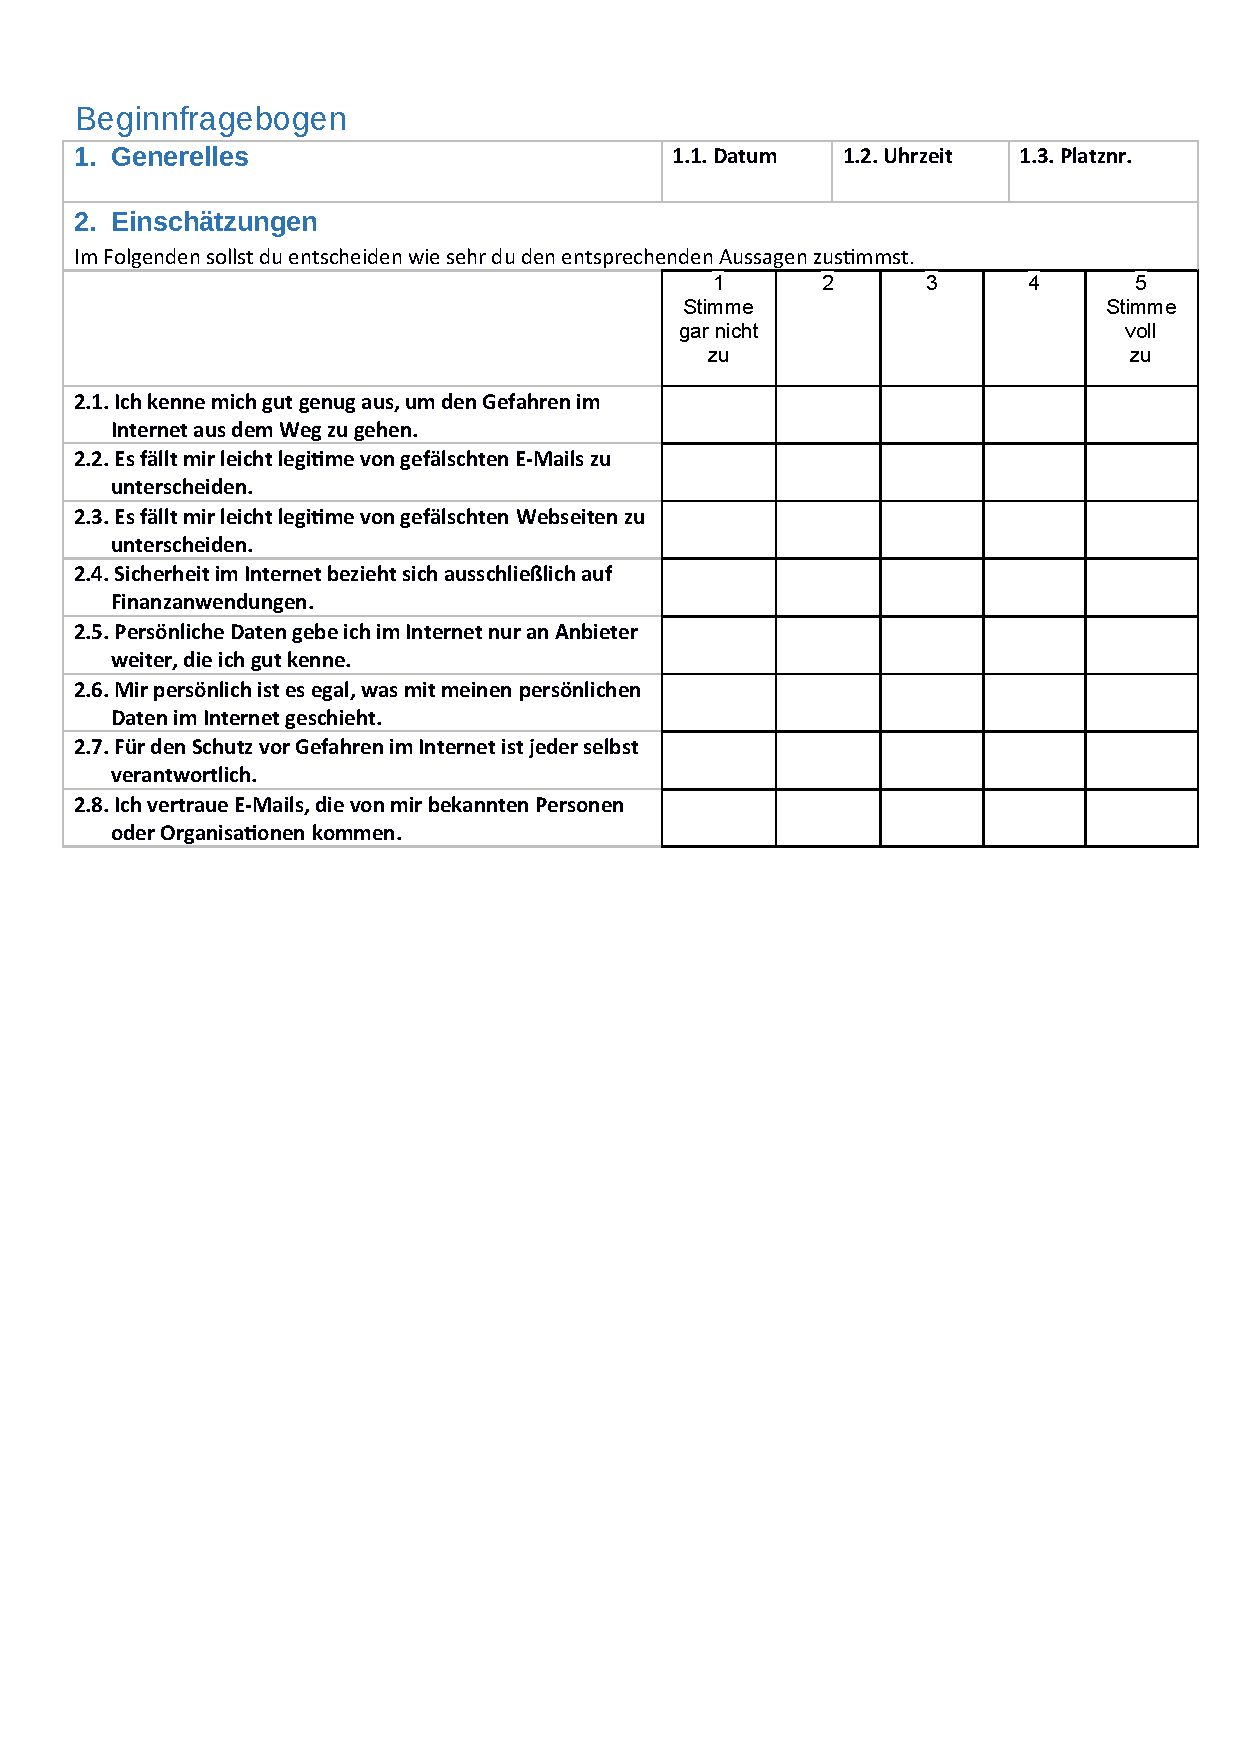
\includepdf[pages=-,frame,scale=0.8]{graphix/before_survey.pdf}
\label{s:url_survey}
\includepdf[pages={1,10},frame,scale=0.8]{graphix/url_survey.pdf}
\label{s:after_survey}
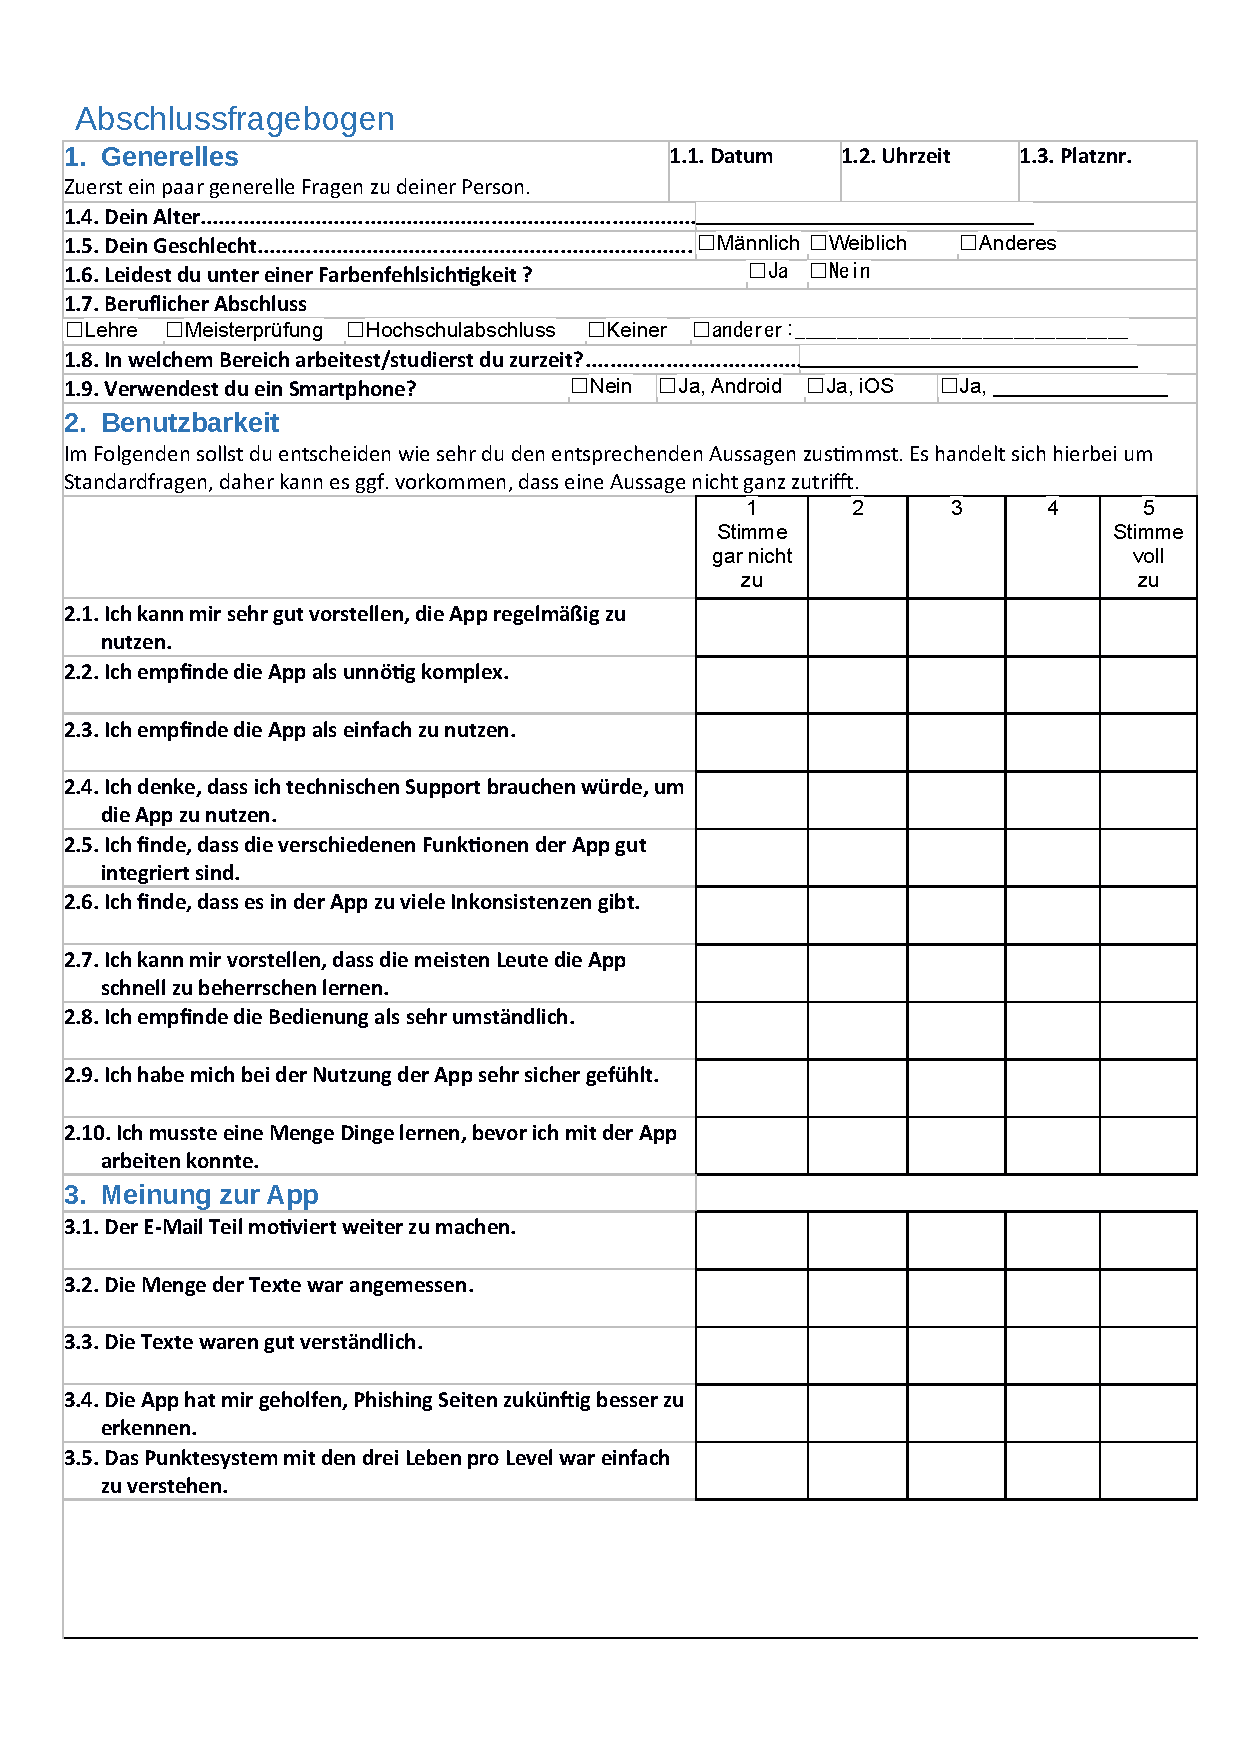
\includepdf[pages={1},frame,scale=0.8]{graphix/after_survey.pdf}

\subsubsection{example URLs before}
\label{example_urls_before}
\begin{itemize}
\item \url{https://plus.google.com/u/0/me}
\item \url{https://www.facebook.signin.com/Raumzeit}
\item \url{http://m.youtube.com/watch?v=Ctzc8QSF6mQ}
\item \url{http://www.amazon.de/Angebote/b/ref=cs_top_nav_gb27?ie=UTF8&}
\item \url{http://130.83.162.6/wiki/Wikipedia:Hauptseite}
\item \url{http://www.ebay.de/rpp/Deals/reisen-gutscheine/stadte-kultur/}
\item \url{https://web.de.myponyfarm.com/}
\item \url{http://abo.net/www.focus.de/digital/}
\item \url{http://www.gmx.net/produkte/mail/promail/}
\item \url{http://de.yahoo.com/?p=us}
\item \url{https://www.ott0.de/damenmode/kategorien/anzuege-kostueme}
\item \url{http://windows.mircosoft.com/de-de/windows/products}
\item \url{http://badcat.com/mobile.twitter.com/session/new}
\item \url{https://touch.www.linkedin.com/login.html}
\item \url{http://m.spiegel.de/panorama/leute/a-937125.html#spRedir}
\item \url{https://www.paypal-sicher.com/webapps/merchantboarding/web}
\end{itemize}


\subsubsection{example URLs after}
\label{example_urls_after}


http://www.amazon.de/Angebote/b/ref=cs_top_nav_gb27?ie=UTF8&

http://www.gutefrage.net.events-ma.de/tag/freizeit/1

http://www.t-online.de/wetter/europawetter/64077226

http://www.immobilienscout25.de/de/finden/wohnen/index.jsp

http://www.ebay.de/rpp/Deals/reisen-gutscheine/stadte-kultur/

http://de.yahoo.com/?p=us

https://130.83.162.6/signup/

https://plus.google.com/u/0/me

http://abo.net/www.focus.de/digital/

http://epaper.bild.de/

https://www.facebook.signin.com/Raumzeit

http://www.welt.de/sonderthemen/mittelstand/forschung/

https://web.de.myponyfarm.com/

http://windows.mircosoft.com/de-de/windows/products

http://www.gmx.net/produkte/mail/promail/

https://mail.live.dub123.com/login.srf?wa=wsignin1.0&rpsnv=12

http://m.youtube.com/watch?v=Ctzc8QSF6mQ

https://www.ott0.de/damenmode/kategorien/anzuege-kostueme/

http://130.83.162.6/wiki/Wikipedia:Hauptseite

https://www.paypal-sicher.com/webapps/merchantboarding/web

https://touch.www.linkedin.com/login.html

http://m.spiegel.de/panorama/leute/a-937125.html#spRedire

http://badcat.com/mobile.twitter.com/session/new

https://blog.xing.com/category/german/


\subsection{Anti-Phish Certificates for Study Participants}
\label{s:antiphish_certs}


\includepdf[pages={1},frame,scale=0.8]{graphix/zertifikat_gold.pdf}

\includepdf[pages={1},frame,scale=0.8]{graphix/zertifikat_silber.pdf}
